\documentclass[11pt]{exam}
\usepackage[margin=1in]{geometry}
\pagestyle{plain}
\usepackage{amsmath,amsfonts,amssymb,amsthm,enumerate}
\usepackage{multicol}
\usepackage[]{graphicx}
\usepackage{hyperref}
\usepackage{tikz}
\usepackage{pgfplots}
\usepackage{subfigure}
\usepackage[final]{pdfpages}

\addtolength{\footskip}{2\baselineskip} % to lower the page numbers
\title{\vspace{-0.5in} Math 115 \\ Worksheet Section 2.1}
\date{}


% \theoremstyle{definition}
% \newtheorem{problem}{Problem}
\renewcommand{\questionlabel}{\textbf{Problem~\thequestion.}}
%\printanswers

\begin{document}
\maketitle
\vspace{-0.75in}
\begin{questions}
  \question (2.1 \#24) The graph of \(f(t)\) gives the position of a
  particle (in meters) at time \(t\) (in seconds). List the following quantities in order,
  smallest to largest.\\
  \begin{minipage}{0.4\linewidth}
    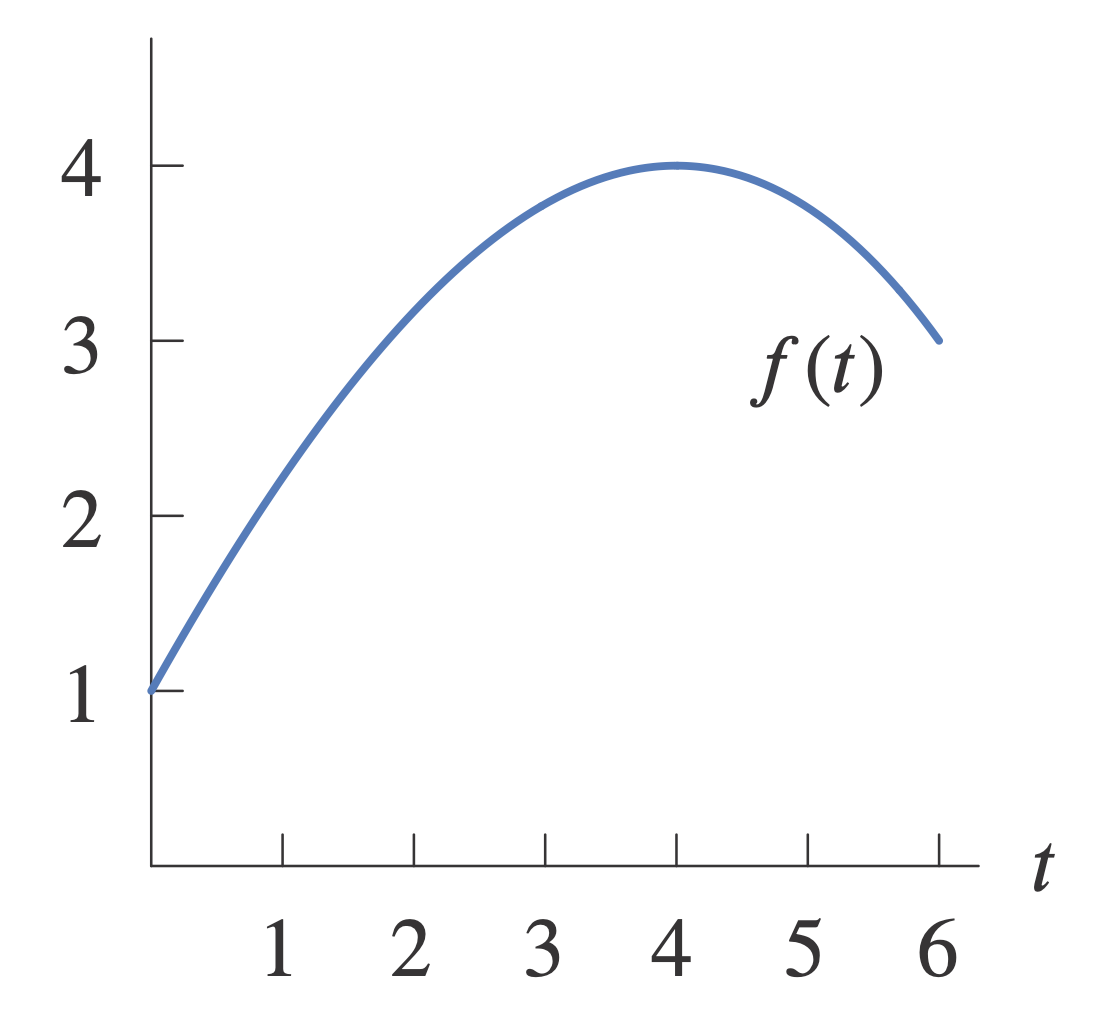
\includegraphics[scale=0.3]{no24graph.png}
  \end{minipage}
  \begin{minipage}{0.6\linewidth}
    \begin{enumerate}[(a)]
    \item The average velocity between \(t=1\) and \(t=3\),
    \item The average velocity between \(t=5\) and \(t=6\),
    \item The instantaneous velocity at \(t=1\),
    \item The instantaneous velocity at \(t=3\),
    \item The instantaneous velocity at \(t=5\),
    \item The instantaneous velocity at \(t=6\).
    \end{enumerate}
  \end{minipage}
  \begin{solution}
    We do not need to estimate the values here, but rather just draw
    lines and see how their slopes compare.\\
    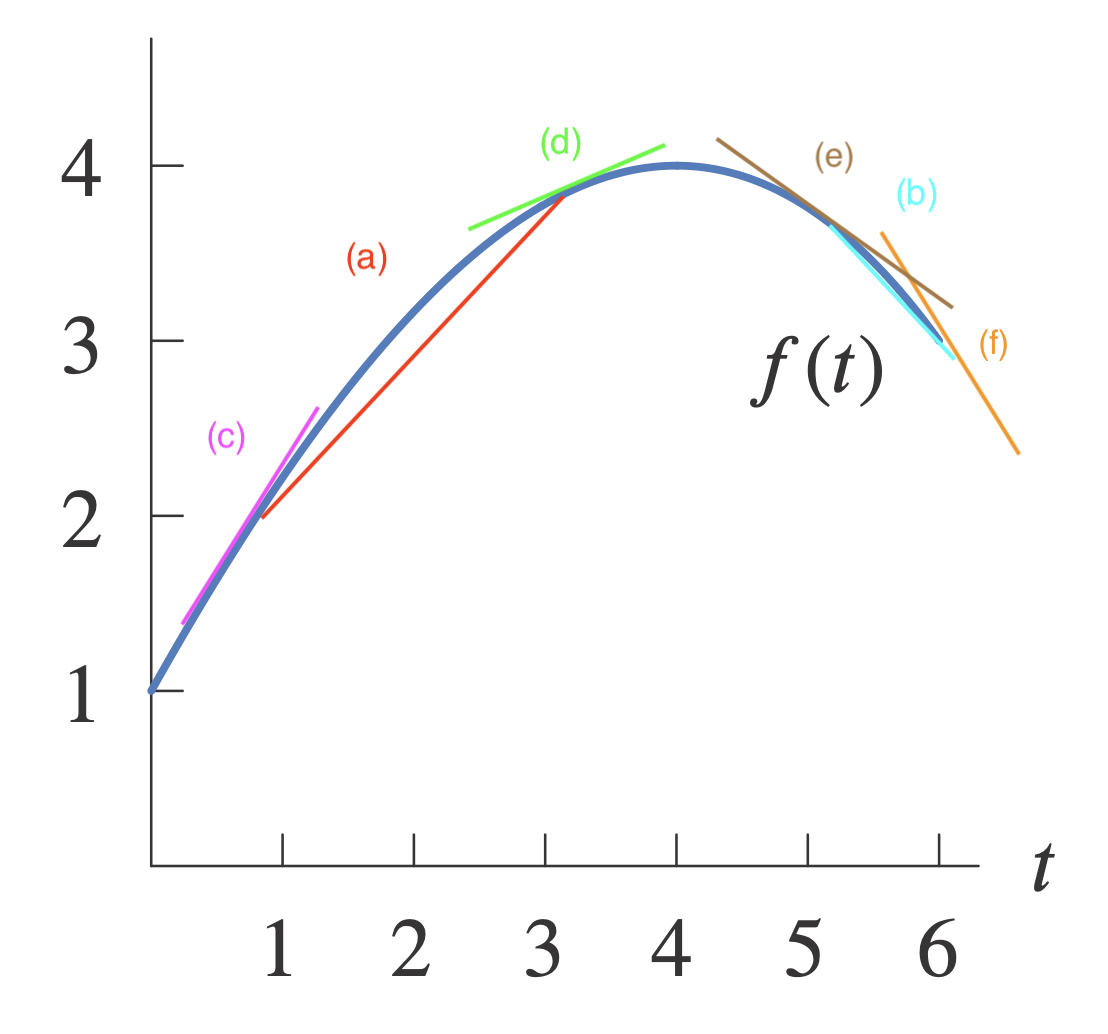
\includegraphics[scale=0.5]{no24graph_with_lines.png}\\
    We see that the slopes of the corresponding lines are in the order
    (f), (b), (e), (d), (a), (c) from smallest to largest.
 \end{solution}
  \question (2.1 \#27)
  A particle moves at varying velocity along a line and \(s=f(t)\)
  represents the particle's distance from a point as a function of
  time, \(t\). Sketch a possible graph for \(f\) if the average
  velocity of the particle between \(t=2\) and \(t=6\) is the same as
  the instantaneous velocity at \(t=5\).
  \begin{solution}
    There are many answers. Here is one.\\
    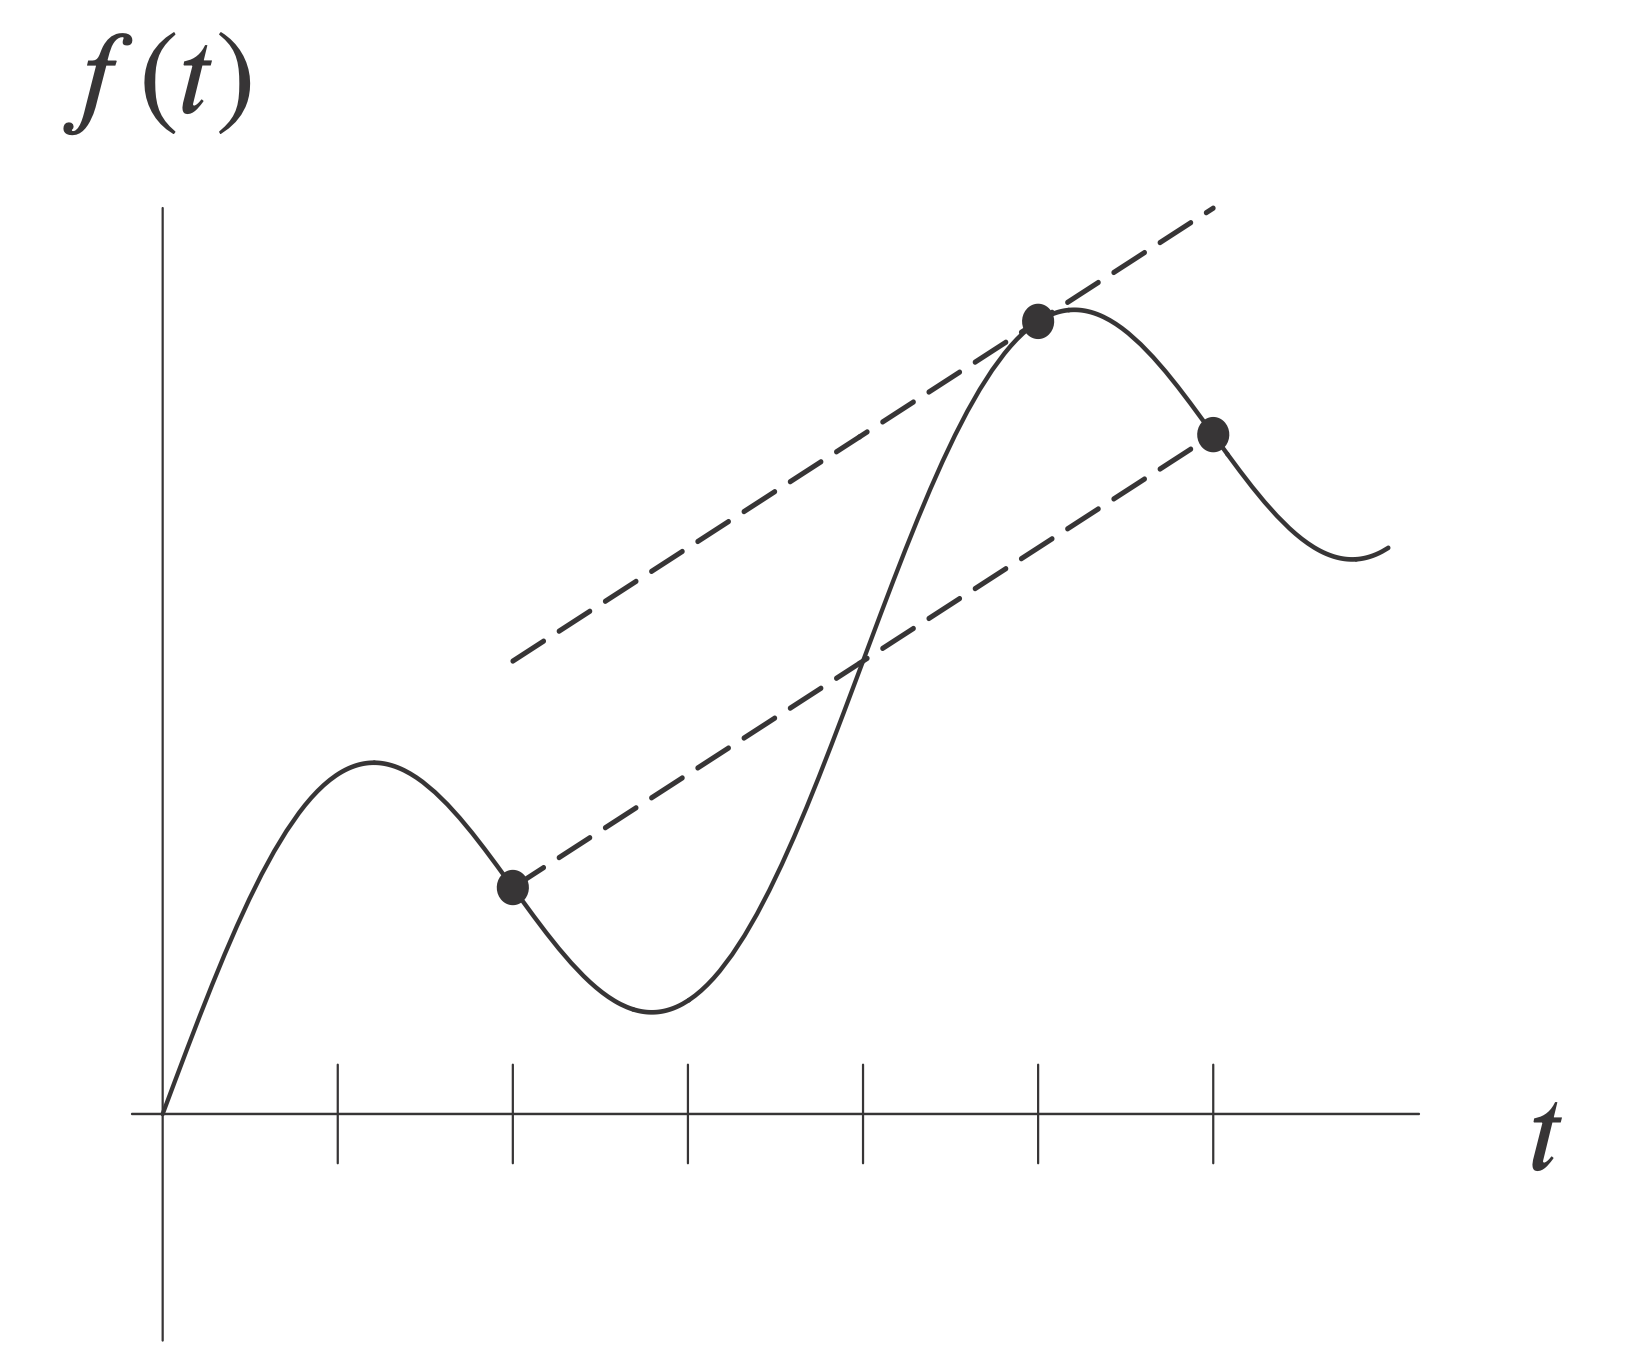
\includegraphics[scale=0.4]{no27answer.png}
  \end{solution}
  \question (2.1 \#34--37)  Decide whether the following statements are true or false and justify.
  \begin{parts}
    \part If a car is going 50 miles per hour at 2 pm and 60 miles per
    hour at 3 pm then it travels between 50 and 60 miles during the
    hour between 2 pm and 3 pm.
    \part If a car travels 80 miles between 2 and 4 pm, then its
    velocity is close to 40 mph at 2 pm.
    \part If the time interval is short enough, then the average
    velocity of a car over the time interval and the instantaneous
    velocity at a time in the interval can be expected to be close.
    \part If an object moves with the same average velocity over every
    time interval, then its average velocity equals its instantaneous
    velocity at any time.
  \end{parts}
  \begin{solution}
    \begin{enumerate}
    \item False. The car could have stopped in between 2pm and 3pm. 
    \item False. All we know is that the car's average velocity was
      40mph, but we do not know how fast it was going at 2pm.
    \item True. This is because average velocity is measured by a
      secant line, but as the interval for the secant line gets
      smaller, it gets closer to the same slope as the tangent line
      for a point in the interval.
    \item True. In this case, if the average velocity is the same for
      any interval, then the object must move at a constant velocity, so
      its instantaneous velocity must equal its average velocity on
      these time intervals.
    \end{enumerate}
  \end{solution}
\question (Winter 2018 Exam 1)
Tom organizes another meeting of his Science Club, but this time only Anne and John can make it. The meeting is at 2 pm, so they both start walking from their houses to Tom's at 1 pm. At 1:18 pm, Anne realizes she forgot her wallet, so she goes back home to get it before heading over to Tom's house.
Anne’s distance in kilometers, $A(t)$, and John's distance in kilometers, $J(t)$, to Tom's
house t hours after 1 pm are given by the graph and the table below. Assume that
both of them walk along a straight line.\\
\begin{minipage}{0.5\linewidth}
  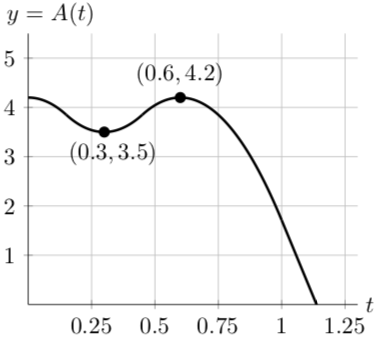
\includegraphics[scale=0.4]{Figures/Tom.png}
\end{minipage}
\begin{minipage}{0.5\linewidth}
$$\begin{tabular}{c|c|c|c|c|c|c} t & 0 & 0.2 & 0.4 & 0.5 & 0.8 & 0.9 \\ \hline J(t) & 5.5 & 4.3 & 3.2 & 2.8 & 0.8 & 0 \end{tabular}$$
\end{minipage}
\begin{enumerate}[(a)]
\item How many kilometers from Tom’s house is Anne's house?
\item Estimate John's instantaneous velocity at 1:24 pm. Show all your computations. Include units.
\item Rank John's average velocity over the time intervals
$$\textrm{(I) } 0.2 \leqslant t \leqslant 0.4 \qquad \textrm{(II) } 0.5 \leqslant t \leqslant 0.9 \qquad \textrm{(III) } 0.8 \leqslant t \leqslant 0.9.$$
\item What was the total distance travelled by Anne?
\item On which of the following intervals is $A(t)$ invertible?
$$\textrm{(I) } [0,0.6] \qquad \textrm{(II) } [0.3,0.6] \qquad \textrm{(III) } [0.1,0.5] \qquad \textrm{(IV) } [0.6,1] \qquad \textrm{(IV) } [0,1].$$
\end{enumerate}
\begin{solution}
  See \href{https://dhsp.math.lsa.umich.edu/exams/115exam1/w18/s3.pdf}{https://dhsp.math.lsa.umich.edu/exams/115exam1/w18/s3.pdf}
\end{solution}
\question 
For the function shown below, at which labeled points is the slope of
the tangent line to the graph positive? Negative? At which labeled
point does the graph's tangent line have the greatest 
(i.e., most positive) slope? The least slope (i.e., negative and with the largest magnitude)?
\begin{figure}[htp]
		\centering
		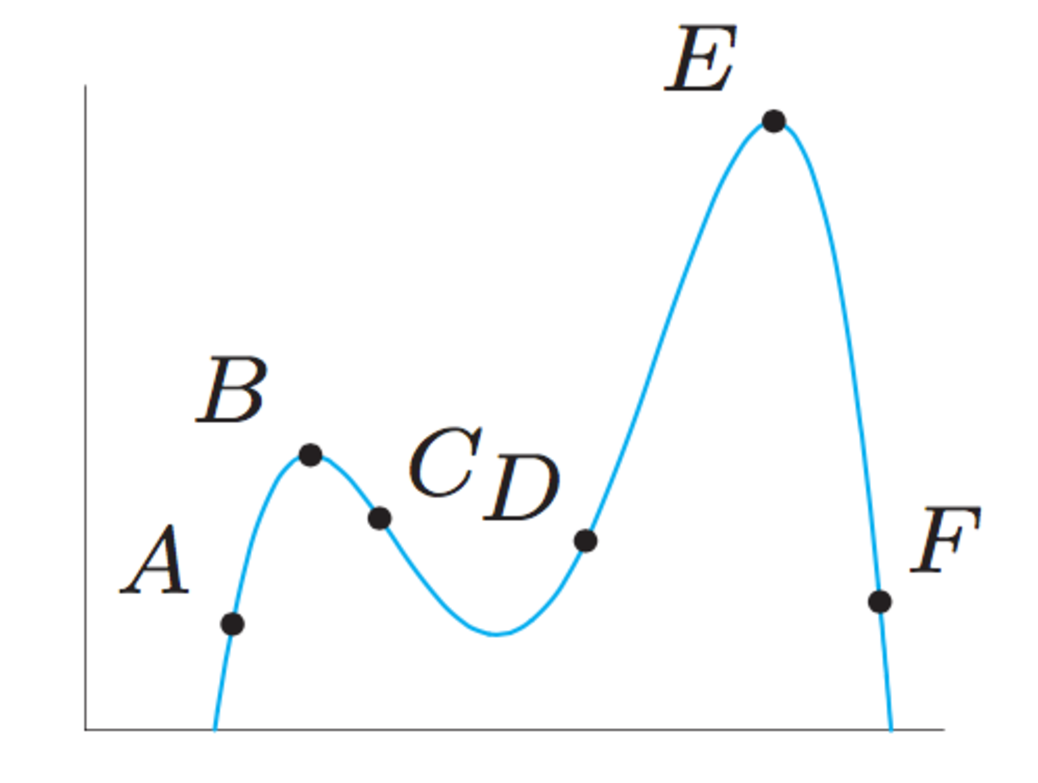
\includegraphics[scale=0.4]{Figures/fig4.pdf}
		%\caption{Graph for Exercise \ref{wash}}\label{fig4}
		\end{figure}
\ifprintanswers \pagebreak \fi
\begin{solution}
  Points where tangent line slope is positive: A,D\\
  Points where tangent line slope is negative: C,F\\
  Point where tangent line slope is greatest: A\\
  Point where tangent line slope is least: F
\end{solution}
\question (Fall 2015 Exam 1) Angelica Neiring and Simona Koloji decide to enjoy the fall weather by racing
each other from the brass block “M” in the center of the Diag along a 2.5 kilometer (2500
meter) route to the Huron River inside the Arb. Let A(t) (respectively S(t)) be Angelica’s
(respectively Simona’s) distance along the route (in meters) t seconds after they start racing.
Angelica and Simona are both wearing GPS watches that record data about their race. The
table of values for the functions A and S below shows some of the resulting data
\begin{tabular}{|c|c|c|c|c|c|c|c|c|c|c|c|c|c|}
  \hline
t&0&30&60&66&72&105&114&120&135&168&180&198&300\\
  \hline
A(t)&0&55&119&137&156&226&249&265&302&384&415&463&737\\
  \hline
  S(t)&0&57&120&137&156&225&248&264&303&389&422&473&768\\
  \hline
\end{tabular}
Use the data above to answer the questions below. Remember to show your work.
\begin{parts}
  \part Estimate Angelica's instantaneous velocity \(3\) minutes into the race.
  \part Estimate Simona's instantaneous velocity \(2\) minutes into
  the race.
  \part Who was ahead 5 minutes into the race?
  \part Who was running faster exactly one minute into the race?
  \part (You may use a calculator on this problem) In describing the race later, Simona says that her average velocity during the
entire race was 2.8 meters per second while Angelica says that after the first 5 minutes,
her average velocity for the rest of the race was 3.1 meters per second.
Assuming their statements and the table of values above are accurate, who won the
race? Or is there not enough information to decide? Explain your reasoning.
\end{parts}
\begin{solution}
  For part (b), we compute average velocity between 114 seconds and
  120 seconds:
  \[\frac{S(120)-S(114)}{120-114}
=\frac{264-248}{6}
= \frac{16}{6}
\approx 2.67 \text{m/s}
\]
We also compute the average velocity between \(120\) seconds and
\(135\) seconds:
\[\frac{S(135)-S(120)}{135-120} =
\frac{303-264}{15}=\frac{39}{15}\approx2.6
\]
So we estimate that the instantaneous velocity at \(120\) seconds is
around \(2.6\) m/s. (Any estimate between the average rates of change
computed above would be reasonable. We rounded to two significant
digits here.)\\
  For the other parts, see
  \href{https://dhsp.math.lsa.umich.edu/exams/115exam1/f15/s2.pdf}{https://dhsp.math.lsa.umich.edu/exams/115exam1/f15/s2.pdf}
\end{solution}
\end{questions}
\end{document}
%%% Local Variables:
%%% mode: latex
%%% TeX-master: t
%%% End:
